\section{Functional block checks}

% Here present a new methodology that was developped, explain why
This section details a concept for a methodology that could help detect and investigate soft-failure more efficiently and robustly.
It has also a broader scope of application than just the search of functional weaknesses, and can help finding errors and design issues during the design phase.
This methodology remained at the concept phase and went only through very early preliminary testing, because it needs a deep involvement of a design team which could not be done during this research work, and potentially some modification of the simulation engine.
It was conceived very late in the research work with the experience and feedback gained from the other modeling methods.

% Speak about virtual test ?
% Speak about per-block validation by running simulation and checking waveforms ?

% Why is it interesting for ESD simulations
Powered-on \gls{asic} simulations are difficult to investigate because of the scale factor inherent to automotive \gls{asic} detailed in the chapter introduction.
\gls{asic} are very dense and complex devices, with multiple levels of hierarchy.
Disturbances propagate through the hierarchy, vertically from top-level down to transistor-level and horizontally between cells.
In case of failure, there can be multiple places where a fix could be applied.

% High level view of the new method
This section details a design method to detect functional failures early during the \gls{asic} design phase.
It is a bottom-up method like the one described in \ref{sec:bottom-up-modeling}.
However, the proposed method focuses on the signals inside the block itself, and not the signals at its boundaries.
The concept is to define for each block function a series of assertions.
An assertion is a condition that raises a flag if not respected.
For a given cell circuit, the designer will define a set of assertions that seem significant in regard of the circuit.
Them, each time the block is instantiated into a testbench and simulated the simulator checks all of the block's assertions at each timestep.
If an assertion goes false, it is recorded in a log along with a timestamp for later analysis.
At the end of an \gls{esd} simulation for instance, the log can be inspected to see what assertions and blocks turned false and at which time.

% Example
For instance, a designer may define a set of assertions for a current mirror \ref{fig:ex-current-mirror-assert}.
He defines that the potential across the gate voltage of a current mirror must be superior the MOS gate threshold.
An assertion is also added to check that the copied current matches the input current.
Another interesting assertion consists in checking that the ground pin voltage never becomes superior to a threshold.
In case a ground pin is misconnected inside a circuit and is floating, its potential will increase above the threshold and this issue will immediately be caught by the assertion checker.

\begin{figure}[!h]
  \centering
  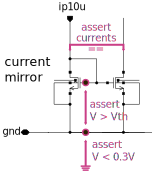
\includegraphics[width=0.5\textwidth]{src/4/figures/example_assertion_current_mirror.pdf}
  \caption{Example schematic with special checking cells}
  \label{fig:ex-current-mirror-assert}
\end{figure}

% Difference with normal verif + validation flow
This method differentiates from virtual testing and validation flow by two key parameters.
In a normal flow, it is the waveforms produced by a block when exposed to stimuli that is being checked.
Those checks are specific to a given simulation and are not reusable.
Here, the assertions are specific to a cell and not to a simulation.
They are reusable, while now IP blocks of analog circuitry tend to become more common.
Also, standard verification can involve setting verification criteria on the waveforms generated by a block during simulation.
In case the produced waveform goes outside those criteria, a simple fail is notified.
Here, the fail is timestamped is essential because it shows not only that something went wrong, but also when and for how long.
It differentiates from normal tooling used during circuit verification to ensure that a block is running properly.

\begin{figure}[!h]
  \centering
  \includegraphics[width=0.3\textwidth]{src/4/figures/special_cells_concept.pdf}
  \caption{Example schematic with special checking cells}
  \label{fig:ex-special-cells}
\end{figure}

% Knowing which flags were raised
Knowing which blocks have raised flags shows where the ESD had an impact.
As a remainder, this method targets complex integrated circuit designs with multiple levels of hierarchy.
For a human being it is a very time-consuming to inspect most nets and blocks manually in order to detect signals and blocks in error.

% Knowing when a flag starts
As indicated earlier, the assertions are timestamped, meaning that the beginning time and end time are recorded.
Failures can be sorted with their beginning time by ascending order.
This sorted list indicates which block went into failure first, and in which order they were all impacted.
It gives a complete picture of the propagation of the disturbance through the complete system.

% Knowing how long a flag was raised
The duration of a flag provides an indication of its severity.
For instance, any flag that is a thousand times shorter than the original \gls{ESD} discharge indicates a very minor fault.
On the contrary, any flag that lasted larger than the discharge should indicate a very severe disturbance, and an aggravation of the original disturbance.

% Combined value of all this information
Combined together, those information enable to make smart decisions about where to fix the issues.
Blocks that are the most sensitive can be easily identified for hardening.

\begin{figure}[!h]
  \centering
  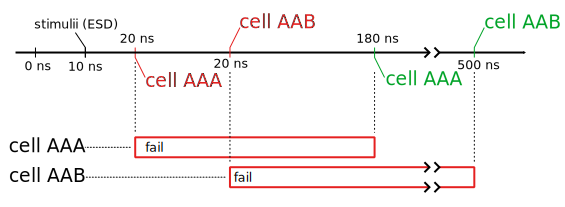
\includegraphics[width=\textwidth]{src/4/figures/example_assertion_analysis.pdf}
  \caption{Example of time chart for investigating failures raised by assertions}
  \label{fig:ex-special-cells}
\end{figure}


\subsection{Implementation}

These assertions can be implemented in different manners.

% Method using spectre-simulator checkers
The Spectre simulator offers the possibility to build a list of assertions to check for a simulation.
This is not exactly the concept described in this section, because this list cannot be associated to a block but only to a simulation.
It can however enable to test this assertion system and the value of information obtained with it.

% Method using a dedicated view
Another option is to create a dedicated assertion view inside the block's cell.
This view takes the form of a text file containing a list of all assertions for the block.
Then, the simulator must be instructed to use this view if it exists and check the assertions defined in it.
% Fig with schematic and assertion file OR schematic with assertion file in it ?

% Method using in-schematic assertions
The last approach is to add directly in the schematic assertion cells (Fig. \ref{fig:ex-special-cells}).
Those cells can be implemented in any analog or mixed-signal \gls{hdl}, such as Verilog-A or VHDL-AMS.
Those cells are transparent for the simulator and do not impact the electrical simulation.

% Example Verilog-a code for special cell amplitude threshold cross ?
% Example Verilog-a code for current detection ?

\begin{figure}[!h]
  \centering
  \includegraphics[width=0.3\textwidth]{src/4/figures/special_cells_concept.pdf}
  \caption{Example schematic with special checking cells}
  \label{fig:ex-special-cells}
\end{figure}

\begin{figure}[!h]
  \centering
  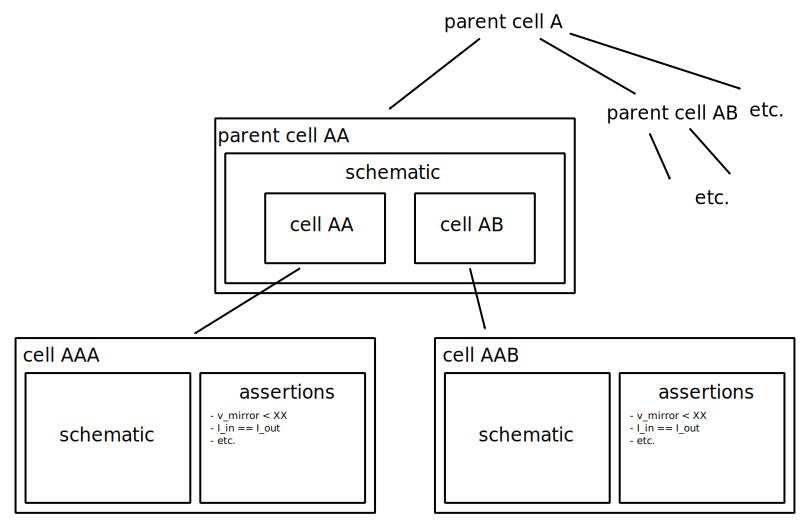
\includegraphics[width=0.7\textwidth]{src/4/figures/architecture_a_assertion.pdf}
  \caption{Cell hierarchy with assertions stored in a file within each bottom cell}
  \label{fig:ex-special-cells}
\end{figure}

\begin{figure}[!h]
  \centering
  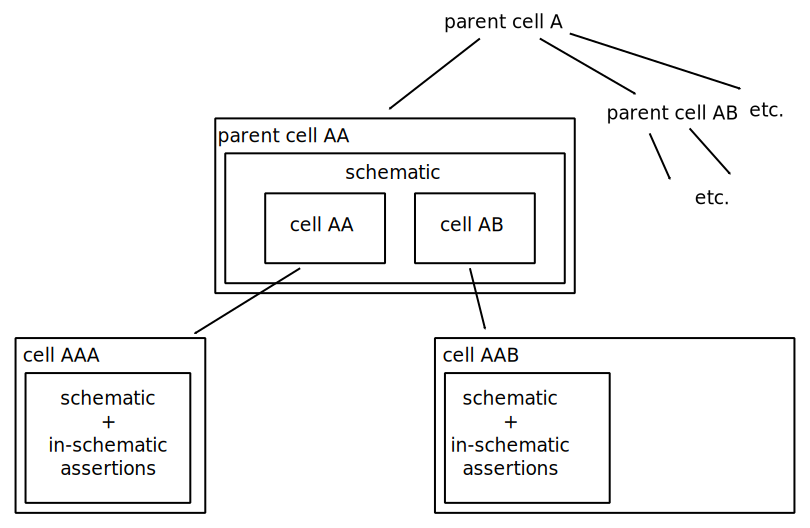
\includegraphics[width=0.7\textwidth]{src/4/figures/architecture_b_assertion.pdf}
  \caption{Cell hierarchy with assertions stored directly inside the schematic of each bottom cell}
  \label{fig:ex-special-cells}
\end{figure}


% Comparison
Each method offers advantages and has inherent defaults.
Using the per-simulation assertions is fast and easy, but it must be repeated for each simulation.
It is not viable for implementing the proposed method.

On the contrary, the assertion view fits well into existing Cadence workflow.
Assertion views can be added to existing schematics without modification.
However, during the design phase, a block gets modified multiple times and by different people.
As a consequence of those modifications, old nets are removed, new nets are created and existing nets can be renamed.
For the assertion view to be useful, it would require designers to update it each time the schematic has been modified.
This extra amount of work, and requiring a designer to modify data in two places tend to indicate that an assertion view is not practical either.

The in-schematic assertions is the most designer-friendly solution.
Designers can easily create assertions between nets, modify them and remove them.
Overall, this option seems to be the most viable.

\subsection{Proof of concept}

% What is the study-case
The concept is tested in a first simulation.
The goal is to show with just a few assertions, the failure case of section \label{sec:failure-case-study} could have been understood more easily and quickly.

% What assertions
Only a few assertions are implemented per block.
The supplies and ground pins are checked against a voltage range.
Current mirrors are checked to ensure current is properly copied.
% What else ?
% Table of assertion placements ?

% How is it checked
The Spectre simulator assertions are used for testing purposes.
% show the circuit ?
A XX V XX ns TLP pulse is injected on VBATT.
Failure is observed on V2p5

The assertions were recorded and given in table XXX


\subsection{Assertion writing}

Assertions are written logically based on the design of the block.
If for instance a net is the gate command of a current mirror, a few criteria can be derived logically.
For the current mirror to function properly, at least 1 gate voltage is required for biasing.
Going below this voltage, the current mirror will not perform its copy anymore.

SCHEMATIC SIMPLE CURRENT MIRROR

Another example is taking a regulator.
If current drawn on the output of the regulator exceeds nominal capability, then the block will be considered faulty.

A set of simple rules could also be derived on supplies and ground.
For all blocks, supplies should be expected within a given range.
Grounds should be expected close to 0, and most likely lower than a body diode triggering voltage.

The second major advantage is that the rules are specific to a block.
They do not depend on boundary blocks, because they focus on the logical behavior of the block itself.
This means that this approach is highly modular and scalable.
Indeed, a set of rules written with an IP block can travel with it.
In any project/IC the block will be used, the rules will apply.

TALK ABOUT VIRTUAL TEST. DIFFERENCE IS VIRTUAL TEST IS INTERESTED IN INTER-BLOCK RELATIONSHIP ?

\subsection{Applicability beyond ESD simulations}

The main application the assertion approach was imagined for in this work is to detect blocks in failure state,
during an \gls{esd}.

However, this technique can have multiple different applications.
The major interest of these assertions would be to run them in any simulation, not just \gls{esd} simulations.

First, the file containing the assertions constitutes an electrical documentation of the block.
Any designer tasked with upgrading a block developed by someone else will immediately get a view of biasing levels,
expected current capabilities, etc.

Also, in a multi-person IC design team, a single block can be simulated by many different people (designer, verification, esd, etc.).
Those people will write testbenches to put those blocks into different situations.
Almost always, testbenches will take quite some time to be debugged, sometimes involving interaction with the original designer of the block.
Here, the assertion system can help avoid that, by highlighting when a block is not properly biased or operated.
Mistakes in testbenches will be easy to detect and understand, for anyone, without requiring the intervention of the original designer.

Also, some blocks require long startup sequence (slow ramp-up), usually regulators that power digital cells.
Those sequences can take an important simulation time.
Those long sequences are an issue if a testbench tries to validate some functionality after startup.
To overcome this issue, some testbenches immediately put the block into its final DC state (using DC sources instead of ramp-up DC sources).
The problem with this approach is that in some cases the block will not be properly biased.
The assertion can help determine whether or not the block is in its final state and properly started.

Also, assertions can help detect early connection issues.
This is very useful for instance to detect floating ground.
A voltage criteria can be set on all ground nets, that will trigger a failure if a ground voltage exceeds for instance 1V.
This is very useful to detect unconnected nets, which can happen regularly with complex IC blocks that mix power functions, digital, analog
and usually have dedicated grounds for each domain.

Potential integration in Cadence environment
So far, limited support for assertions in Cadence.
In an ideal case, assertion files should be a specific view of the asserted cell.
This way, when the cell is copied or moved around, the assertions will move with it and be reused.

\subsection{Perks and Drawbacks}

Simple to write.
Reusable.
Integrates well into the design flow
General purpose (not limited to ESD, very useful in general considering all applications).

DRAWBACKS ?
Right amount of assertions to write ?
Quality of the issue detection will depend on the quality of the assertions ?
How to assess coverage ?


\subsection{Conclusion and follow-up work}

A new concept that could not reasonably be developed in the timeframe of this research work was presented.
Potential solutions and design choices for building a prototype were presented.
This concept could be developed into a prototype in order to evaluate initial issues.
Topology analysis
